\chapter{Szenarios}

\section{ARP-Spoofing}

\subsection*{Voraussetzungen}

Für diesen Angriff ist Zugang zum Netzwerk des anzugreifenden Hosts notwendig. Ebenso ist es notwendig eine gültige IPv4 Adresse aus diesem Netzwerk zu besitzen.
Der angreifende Rechner benötigt ein Programm um gefälschte ARP Replys zu senden (hier verwendet: Ettercap). Zusätzlich wird Wireshark eingesetzt, da sich der Netzwerkverkehr damit besser analysieren lässt als mit Ettercap.
Um den mitgelesenen Netzwerkverkehr zu manipulieren ist ein funktionsfähiger etterfilter notwendig.

\subsection*{Grundlagen}

\uline{Funktionsweise von ARP}

Mittels ARP (Address Resolution Protocol) kann die physikalische Adresse eines Netzwerkteilnehmers mithilfe dessen IP-Adresse ermittelt werden. Das ist notwendig, um die IP-Pakete in Ethernet-Frames zu verpacken. Will ein Rechner mit einem anderen in einem Netzwerk kommunizieren, wird erst geprüft, ob die MAC Adresse bereits bekannt ist. Hierfür wird die eigene ARP-Tabelle nach einem Eintrag für die Ziel-IP Adresse durchsucht. Ist kein Eintrag vorhanden, sendet der Quellrechner einen ARP-Request(Abb. \ref{fig:arp_request_small}) an die Broadcast-MAC-Adresse um die MAC zu seiner Ziel-IP von den anderen Netzwerkteilnehmern zu erfragen. Daraufhin schickt der Zielrechner seine MAC Adresse mittels eines ARP-Replys(Abb. \ref{fig:arp_reply_small}) direkt an den Quellrechner. Dieser legt für die Kombination aus IP und MAC Adresse einen Eintrag in seiner ARP-Tabelle an. \\
Da es bei Erscheinen von ARP (1982) noch keine Rolle spielte, ob das Protokoll sicher ist oder nicht, sondern nur das es die benötigte Funktionalität liefert, sind dessen Schwächen erst später aufgekommen.\\
\begin{figure}[h!]
	\centering
		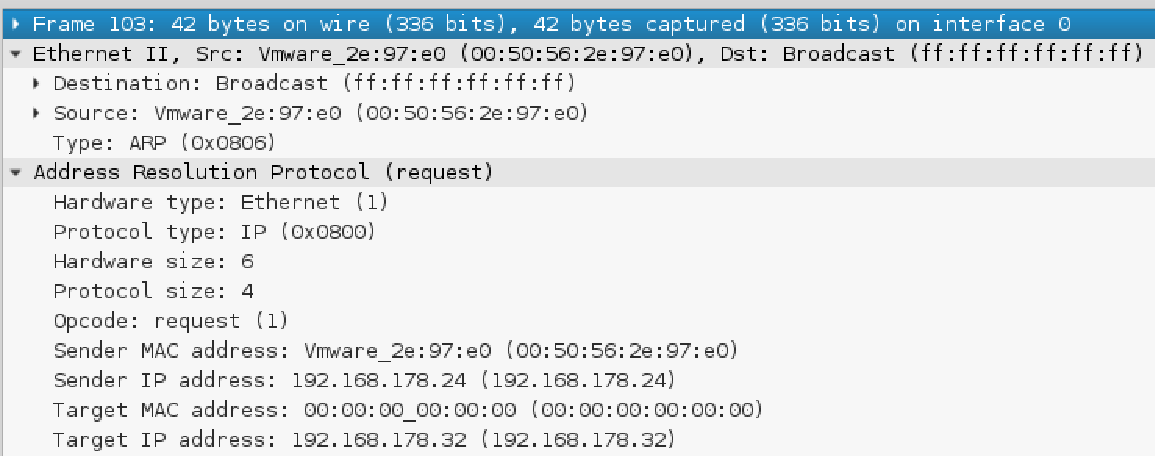
\includegraphics[width=0.80\textwidth]{bilder/arpSpoofing/arp_request_small.pdf}
	\caption{Aufgezeichneter ARP-Request (hier für die Adresse 192.168.178.32)}
	\label{fig:arp_request_small}
\end{figure}

\begin{figure}[h!]
	\centering
		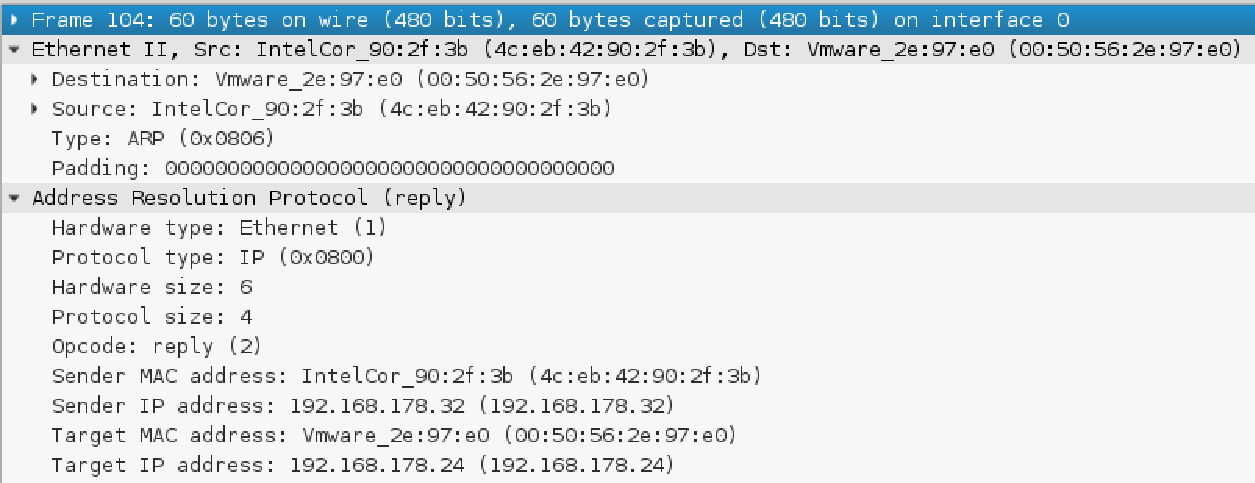
\includegraphics[width=0.80\textwidth]{bilder/arpSpoofing/arp_reply_small.pdf}
	\caption{Aufgezeichneter ARP-Reply (hier von der Adresse 192.168.178.32)}
	\label{fig:arp_reply_small}
\end{figure}



\subsection*{Szenario}
Ein Client eines Netzwerkes möchte mit einem anderen Client kommunizieren. Dafür prüft er in seiner eigenen ARP-Tabelle, ob ein Eintrag (Zuordnung IP <-> MAC) für den Ziel Client existiert. Ist dies der Fall, sendet er seine Daten an die MAC-Adresse des Ziel-Clients. Andernfalls wird die MAC Adresse mittels ARP-Request angefragt.
Der Angreifer macht sich zunutze, dass die meisten Betriebssysteme ARP-Replys ohne Prüfung zulassen. So ist es möglich, die eigene MAC-Adresse den IP-Adressen in der ARP-Tabelle zuzuordnen. Die angegriffenen Clients (einer bis alle eines Netzes) kommunizieren von nun an über den Rechner des Angreifers.



\subsection*{Technisches}
Bei ARP-Spoofing handelt es sich um einen MITM (Man-In-The-Middle) Angriff, mit dem der Netzwerkverkehr zwischen Netzwerkteilnehmern abgehört werden kann.
Der Angreifer „vergiftet“ den ARP-Cache des angegriffenen Rechners um dessen Netzwerkverkehr umzuleiten und mitzulesen/ verändern.

\begin{figure}[h!]
	\centering
		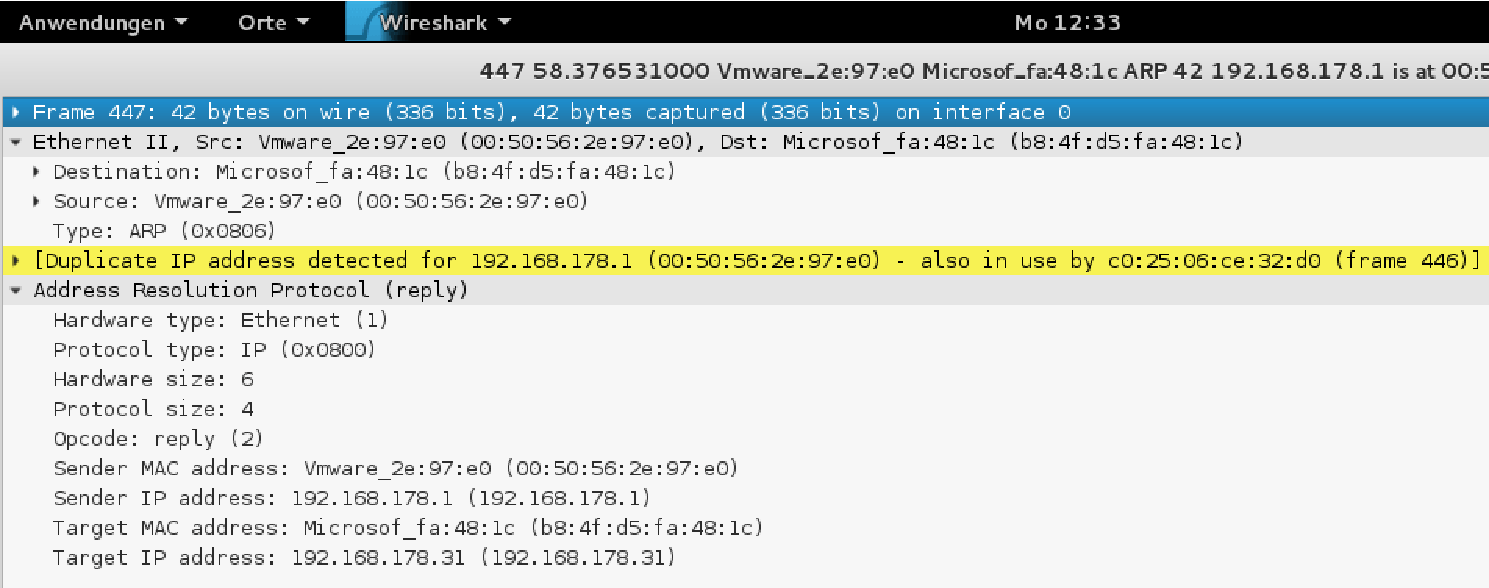
\includegraphics[width=0.80\textwidth]{bilder/arpSpoofing/fake_arp_small.pdf}
	\caption{Aufgezeichneter fake ARP-Reply}
	\label{fig:fake_arp_small}
\end{figure}

\textit{Vorgehen:}
Der Angreifer sendet gefälschte ARP-Replys(Abb. \ref{fig:fake_arp_small}) in das Netzwerk. Diese ARP-Replys teilen den Netzwerkteilnehmern mit, dass die IP-Adressen der anderen Netzwerkteilnehmer (egal ob andere Hosts, Gateway oder andere) über die MAC-Adresse des Angreifers zu erreichen ist. Dies funktioniert, da vom Betriebssystem nicht geprüft wird, ob ein ARP-Reply einen vorausgehenden ARP-Request folgt.

Dieser aufgezeichnete ARP-Reply zeigt, dass dem Ziel (192.168.178.31) mitgeteilt wird, dass das Gateway (192.168.178.1) unter der MAC-Adresse 00:50:56:2e:97:e0 zu erreichen ist. Diese MAC-Adresse entspricht der des angreifenden Rechners.
Das, oder die Opfer, tragen diese Information in die lokalen ARP-Tabellen ein.
\\
\begin{figure}[h!]
	\centering
		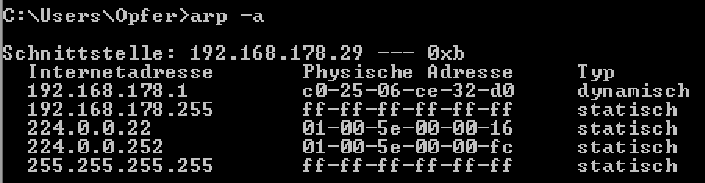
\includegraphics[width=0.80\textwidth]{bilder/arpSpoofing/arp_vorher.pdf}
	\caption{ARP-Tabelle vorher}
	\label{fig:arp_vorher}
\end{figure}

\begin{figure}[h!]
	\centering
		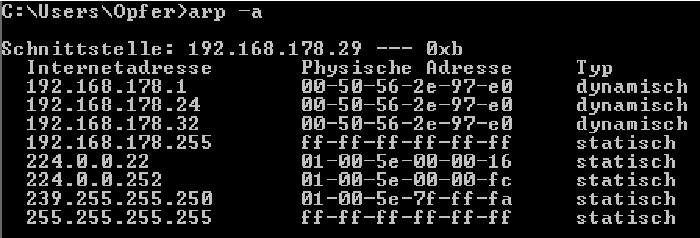
\includegraphics[width=0.80\textwidth]{bilder/arpSpoofing/arp_nachher.pdf}
	\caption{ARP-Tabelle nachher}
	\label{fig:arp_nachher}
\end{figure}

Die beiden Abbildungen \ref{fig:arp_vorher} und \ref{fig:arp_nachher} zeigen, wie die ARP-Tabelle eines angegriffenen Windows Rechners manipuliert wird. Die obere der Abbildungen zeigt den Zustand der ARP-Tabelle vor dem Angriff, mit der korrekten MAC-Adresse des Gateways. Die untere Abbildung zeigt, dass die Adressen 192.168.178.1, 192.168.178.24 und 192.168.178.32 unter der selben MAC-Adresse erreichbar sind.

Sendet das Opfer jetzt Pakete über das Netzwerk, werden diese über den Angreifer umgeleitet und von diesem an das eigentliche Ziel weitergeleitet. Dieses sendet seine Antwort wiederrum an den Angreifer, welcher sie an das Opfer weitergibt. Die Abbildungen \ref{fig:arp_soofing_before} und \ref{fig:arp_soofing_after} zeigen, wie sich die Netzwerkkommunikation während 
Dem Angreifer ist es somit möglich:
\begin{itemize}
	\item Die komplette Netzwerkkommunikation mitzulesen
	\item Die Netzwerkkommunikation zu manipulieren
	\item Einen Denial-of-Service zu erwirken (z.B. Verkehr über Port 80 verwerfen, daraus folgt: keine Kommunikation mit Webserver mehr möglich)
\end{itemize}

\begin{figure}[h!]
	\centering
		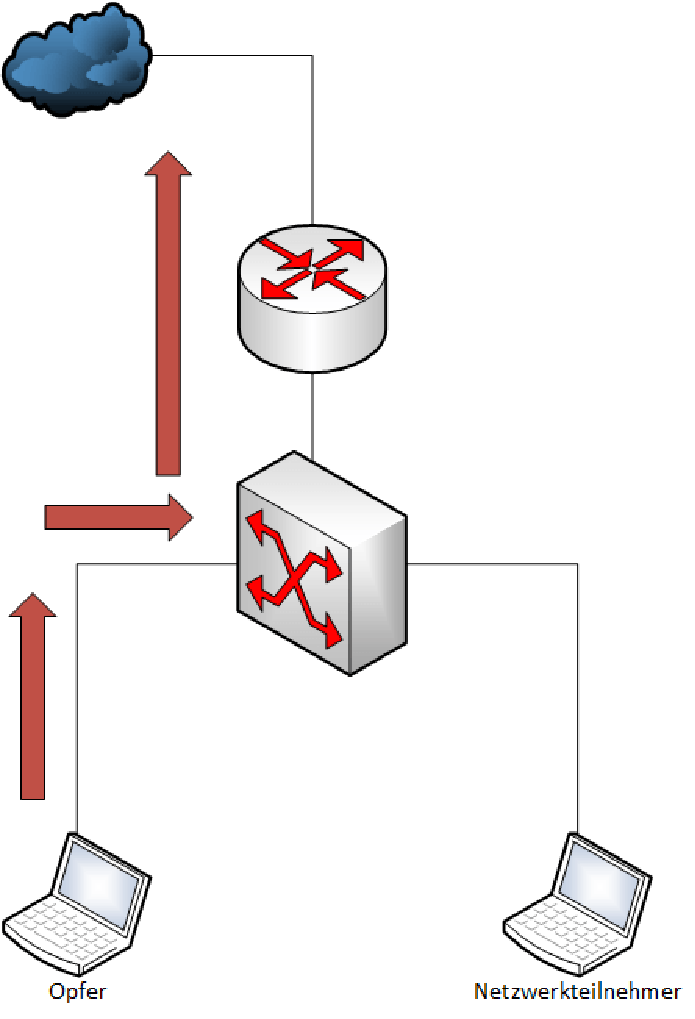
\includegraphics[width=0.40\textwidth]{bilder/arpSpoofing/arp_soofing_before.pdf}
	\caption{Vor dem Angriff: Die Netzwerkkommunikation des Opfers erfolgt über das Gateway des Netzes (bzw. direkt mit anderen Netzwerkteilnehmern)}
	\label{fig:arp_soofing_before}
\end{figure}

\begin{figure}[h!]
	\centering
		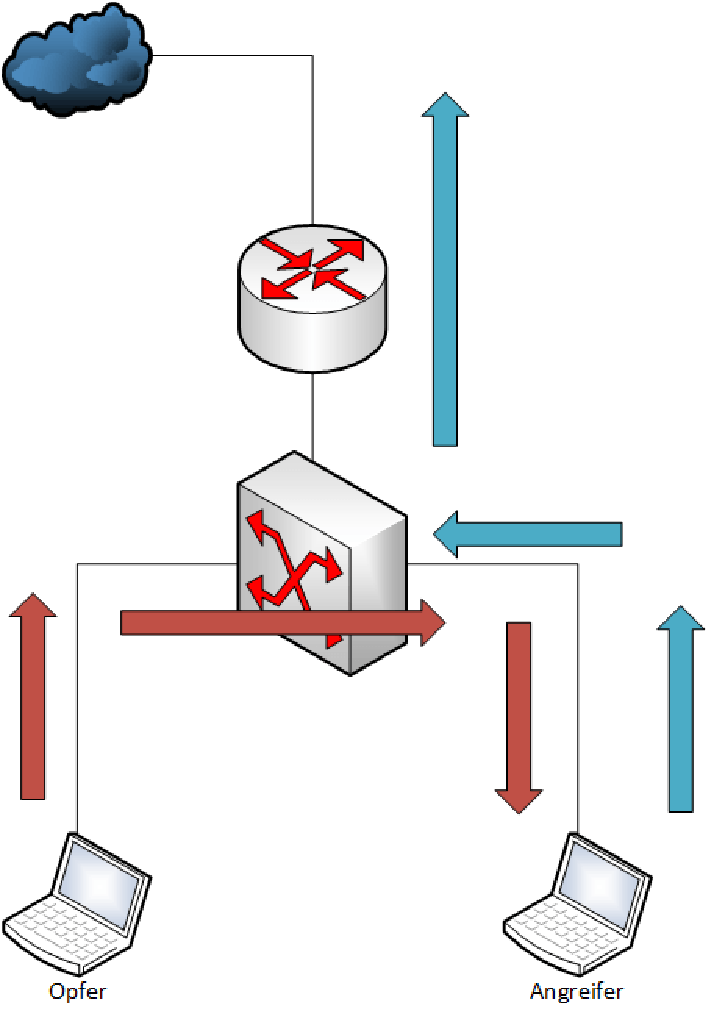
\includegraphics[width=0.40\textwidth]{bilder/arpSpoofing/arp_soofing_after.pdf}
	\caption{Während des Angriffs: Die Netzwerkkommunikation des Opfers erfolgt über den Rechner des Angreifers. Die Kommunikation aus dem öffentlichen Netz in Richtung Opfer (bzw. von anderen Teilnehmern des LANs) erfolgt ebenfalls über den Angreifer (die Pfeile sind hier nur in eine Richtung dargestellt)}
	\label{fig:arp_soofing_after}
\end{figure}


\subsection*{Erklärung der verwendeten Skripte und Tools}

\subsubsection*{Ettercap}

Bei diesem MITM Angriff mittels ARP-Spoofing wird Ettercap zum Senden der gefälschten ARP-Replys verwendet. Ettercap bietet verschiedene Möglichkeiten Angriffe durchzuführen. Für ARP-Spoofing wird der MITM Angriff mittels ARP poisoning verwendet.
Ettercap bietet zusätzlich zur Bedienung über die Konsole ein grafisches Interface. Diese listet alle verfügbaren Ziele auf und der Angreifer kann bequem Angriffe starten.

Der Angriff wird über folgenden Aufruf gestartet:
\lstset{language=bash}
\begin{lstlisting}[
	basicstyle=\footnotesize,
]
ettercap -T -i eth0 -M ARP /Opfer-IP// ///
\end{lstlisting}

Verwendete Parameter:
\begin{itemize}
	\item T: Verwenden des Textinterfaces, der Benutzer kann durchgehend mit h in der Konsole eine Hilfe anzeigen
	\item i: Gibt das Interface an über das der Verkehr umgeleitet werden soll. In obigem Beispiel „eth0“
	\item M: Aktiviert den MITM Angriff. Der folgende Parameter „ARP“ startet den MITM mittels ARP poisoning
	\item Anschließend wird die IP-Adresse des Opfers (oder die Netzadresse des Opfer-Netzes) angegeben. Es können auch mehrere Ziele angegeben werden: /Opfer-IP1//Opfer-IP2/ 
\end{itemize}

\subsubsection*{Etterfilter}
Bei Manipulation der Netzwerkkommunikation wird zusätzlich etterfilter verwendet. Im Beispielprogramm werden Bilder auf Webseiten durch ein anderes Bild ersetzt. Der Filter prüft dabei lediglich, ob im übertragenen Seitenquelltext ein \textit{img src=} vorhanden ist. Ist das der Fall wird dieses mit \textit{img src=Pfad\_zum\_Bild} (Abb. \ref{fig:etterfilter}) ersetzt. Der Alte Bildpfad wird dabei nicht ersetzt, er steht noch immer im img-HTML-Tag, allerdings nicht mehr als Pfadangabe.
\begin{figure}[h!]
	\centering
		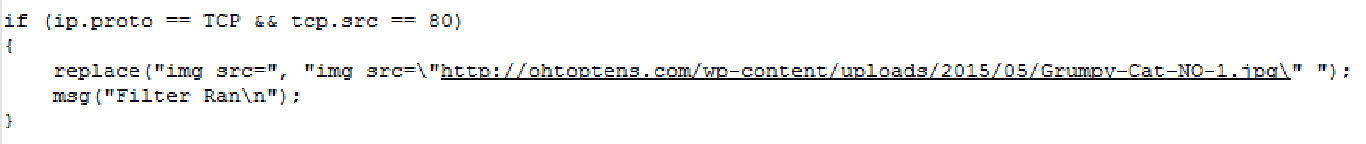
\includegraphics[width=0.90\textwidth]{bilder/arpSpoofing/etterfilter.pdf}
	\caption{Teil des Etterfilters um Bilder zu ersetzen.}
	\label{fig:etterfilter}
\end{figure}

Gestartet wird der Angriff über:
\lstset{language=bash}
\begin{lstlisting}[
	basicstyle=\footnotesize,
]
ettercap -T -F pfad_zum_filter -i eth0 -M ARP /Opfer-IP// ///
\end{lstlisting}

\subsection{Benutzung des Python Skripts}
\begin{enumerate}
	\item Um einen "`normalen"' MITM Angriff zu starten muss im ARP Spoofing Menü Menüpunkt eins gewählt werden. 
	\item Anschließend ist das Interface auszuwählen über welches der Netzwerkverkehr umgeleitet werden soll.
	\item \textit{arp-scan --interface=eth0 -localnet} ermittelt alle angreifbaren IP-Adressen im lokalen Netzwerk, die über das in 2. gewählten Interface erreichbar sind (Abb. \ref{fig:arp_scan}) .
	\begin{figure}[h!]
	\centering
		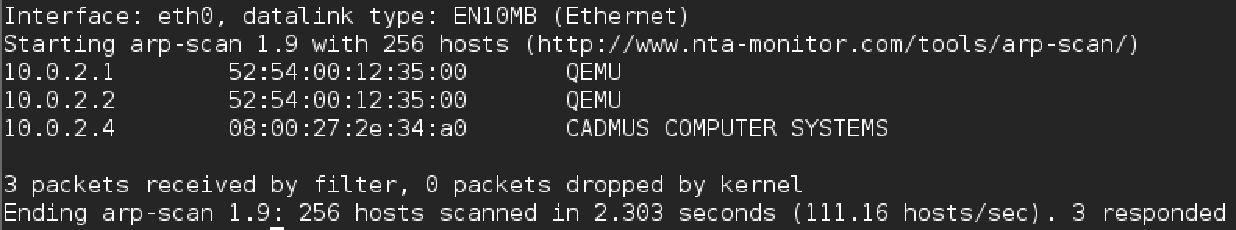
\includegraphics[width=0.90\textwidth]{bilder/arpSpoofing/arp_scan.pdf}
	\caption{Ausgabe von arp-scan.}
	\label{fig:arp_scan}
\end{figure}
	\item Nach Auswahl der anzugreifenden IP-Adresse startet Wireshark. Mit Drücken von Eingabe wird das Programm fortgesetzt und der ARP-Cache des Opfers "`vergiftet"'.
	\item Am Opferrechner kann nun die manipulierte ARP-Tabelle eingesehen werden.
	\item Der Angreifer liest den kompletten Netzwerkverkehr mit.
	\item Pressen von "`q"' beendet den Angriff und stellt die ursprüngliche MAC-Adresse im Cache des Opfers wieder her. 
\end{enumerate}

Die Manipulation des Netzwerkverkehrs kann über den zweiten Menüpunkt gestartet werden. Die Benutzung ist identisch zum „normalen“ MITM-Angriff, mit dem Unterschied, dass Wireshark nicht gestartet wird. Sobald der Angriff läuft kann auf dem Opfer-System eine Webseite aufgerufen werden um zu zeigen, dass Bilder ersetzt wurden (gut geeignet: \url{www.sz.de}).

\subsection{Gegenmaßnahmen}
ARP-Spoofing lässt sich gut erkennen, wenn man sich die ARP-Tabellen der Netzwerkteilnehmer ansieht. Dann fällt auf, dass mehrere IP-Adressen einer einzigen MAC-Adresse zugeordnet sind. Auch über das Sniffen des Netzwerkverkehrs lässt es sich erkennen, da der Angreifer in regelmäßigen Zeitabständen eine Menge ARP-Pakete aussenden muss.
Um das ARP-Spoofing zu verhindern können statische ARP-Tabellen verwendet werden. Der Nachteil dabei ist, dass diese Tabellen dann nicht mehr dynamisch sind und sie für jeden Teilnehmer geändert werden müssen, wenn z.B. ein neuer Netzwerkteilnehmer hinzukommt. Ein wenig mehr Sicherheit bringt es, wenn immerhin die MAC-Adresse des Gateways statisch eingetragen wird.
Besser ist es, Systeme zu verwenden welche den Netzwerkverkehr analysieren und z.B. die ARP-Replys prüfen. So können fehlerhafte und gefälschte ARP-Replys herausgefiltert werden. Beispiele hierfür sind z.B. die Personal Firewalls von Sygate oder SnoopNetCop Pro. Diese melden Angriffe an den Benutzer, die Abwehrmaßnahmen müssen allerdings selbstständig getroffen werden.
Eine weitere Möglichkeit in Linux-Netzwerken ist, dass den Benutzern keine Root-Rechte verliehen werden. Da das Senden von ARP-Replys diese benötigt, kann dies unterbunden werden. Diese Möglichkeit bietet allerdings keinen Schutz vor Angreifern, die einen eigenen Rechner in das Netz einbringen, oder einen Rechner mit einem Live Betriebssystem starten. 


\section{DNS-Spoofing}

\subsection*{Vorraussetzungen}

\begin{itemize}
\item Kali Linux 2.0
\item ARP-Spoofing
\item dnsspoofing
\end{itemize}


\subsection*{Grundlagen}

\subsubsection*{DNS}
Die Addressierung und der anschließende Verbindungsaufbau zu einem Server erfolgt über eine eindeutige IP-Adresse. Damit der Mensch leichter eine Verbindung zu einem Server aufbauen kann,
wurde das DNS (Domain Name System) eingeführt. Dieses verwendet so genannte Domains zur Idenitifzierung von Servern, beispielweise "www.thi.de", da sich diese leichter merken lassen, als
eine IP-Adresse (z.B. 194.94.240.179). DNS ähnelt damit der Funktionsweise eines Telefonbuchs.
Das Domain Name System ist baumförmig aufgebaut, wie nachfolgende Abbildung \ref{fig:dns} illustriert: \\
\begin{figure}[h!]
	\centering
	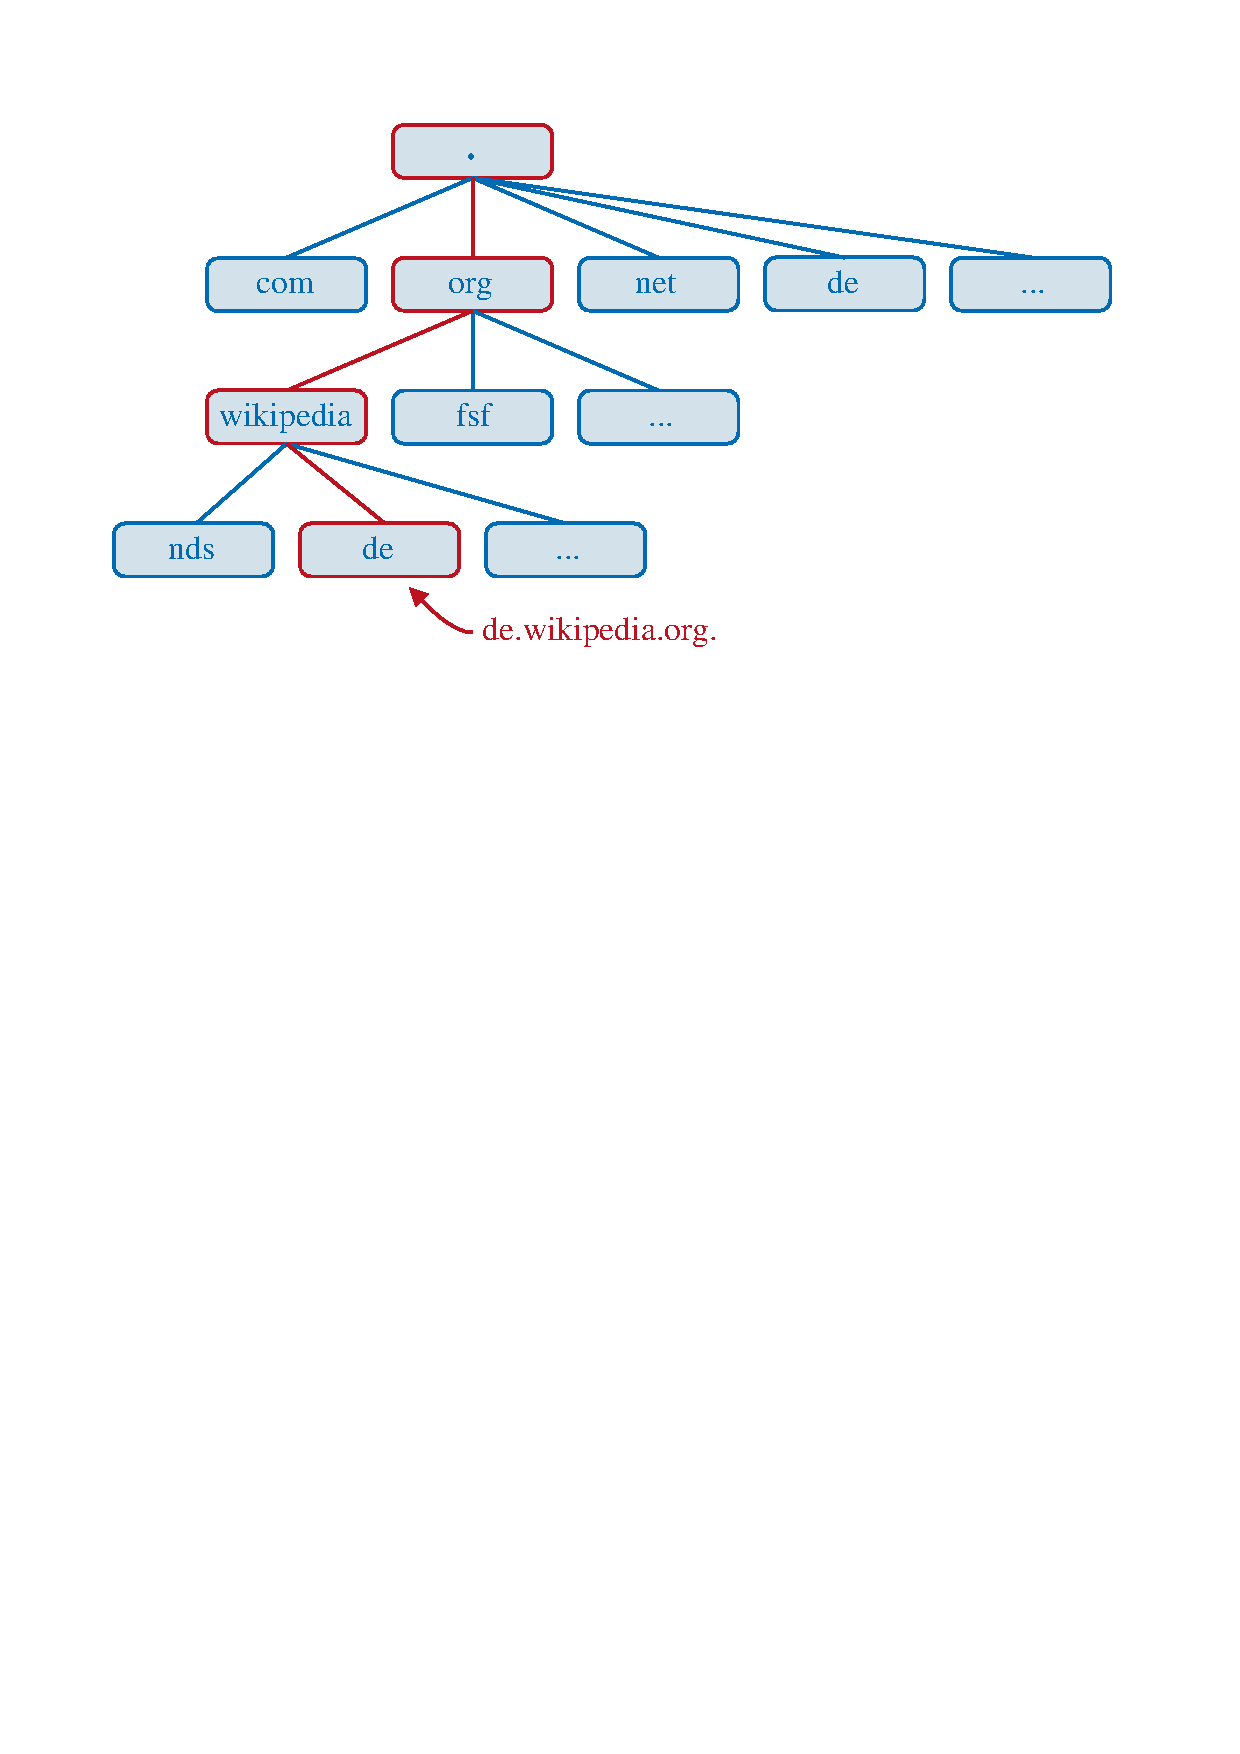
\includegraphics[width=0.7\textwidth]{bilder/dns.pdf}
	\caption{Aufbau DNS \cite{dnspicture}}
	\label{fig:dns}
\end{figure}

%[https://de.wikipedia.org/wiki/Domain_Name_System#/media/File:Dns-raum.svg]


\subsection*{Szenario}
Ein Client (z.B. Windows-Rechner) möchte die Internetseite der Technischen Hochschule Ingolstadt (www.thi.de) aufrufen. Dazu stellt dieser einen DNS-Request an seinen lokalen DNS-Server.
Wenn dieser in seinem Cache keinen Eintrag findet, frägt er - beginnend am Root-DNS-Server - iterativ alle Nameserver nach ihren Einträgen ab, um zum Schluss die IP-Adresse von www.thi.de
zu erhalten.\\
\begin{figure}[h!]
	\centering
	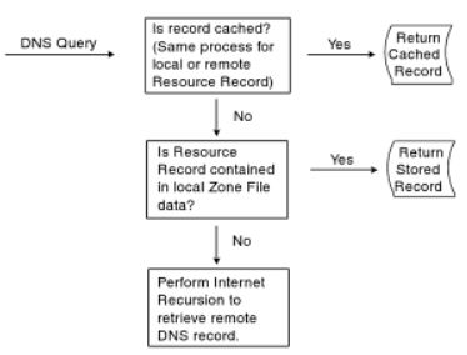
\includegraphics[width=0.7\textwidth]{bilder/DNS-Request.pdf}
	\caption{Ablauf DNS-Anfrage \cite{young2003hacker}}
	\label{fig:dnsrequest}
\end{figure}
%Abbildungs-Quelle: The Hacker's Handbook: The Strategy Behind Breaking into and Defending Networks - Seite 335

\subsection*{Technisches}
Um einen DNS-Eintrag für eine Domain, beispielsweise www.thi.de, zu manipulieren, kann mittels DNS Cache Poisoning der lokale DNS-Cache des Clients mit falschen Einträgen "vergiftet" werden.
Da bei jeder DNS-Anfrage eine zufällig generierte Transaktions-ID mitgeschickt wird, und eine DNS-Antwort nur akzeptiert wird, wenn diese mit der Anfrage übereinstimmt, muss man als Angreifer diese ermitteln, was sich in einem lokalen Netzwerk mit einem Sniffer sehr einfach realisieren lässt. Alternativ kann auch die Transaktions-ID erraten werden, wofür für die 16-Bit lange Transaktions-ID im Durchschnitt 32.768 Versuche notwendig sind.

\subsection*{Tools}
DNSSpoofing wurde von Dug Song \footnote{Diese und weitere Tools von Dug Song sind unter \url{www.monkey.org/~dugsong/dsniff} erhältlich.} entwickelt und veröffentlicht. Mit Unterstützung dieses Tools ist ein Manipulation des DNS-Caches eines Clients im lokalen
Netzwerk sehr leicht durchzuführen. Das Tool ermittelt die verwendeten Transaktions-ID durch Sniffen der ID, wenn der DNS-Server versucht eine Antwort an den Client zu übermitteln. Sobald er die ID der
Anfrage ermittelt hat, muss er eine schnellere Antwort an den anfragenden Client versenden, als der eigentliche DNS-Server. Dies geschieht in mehrfachen Tests und Analysen durch Wireshark regelmäßig. \\

\subsection*{Benutzung von DNS-Spoofing-Skript}
Um dnsspoof einsetzen zu können, muss initial eine hosts-Datei erstellt werden, die die zu manipulierenden Einträge in folgendem Format enthält: \newline

\begin{lstlisting}[caption=Beispiel für eine Hosts-Datei]{Name}
<IP-Adresse>		<Domain>
<192.168.20.135>	www.thi.de
(Wichtig ist hierbei die Trennung von IP-Adresse und Domainname durch Tab und keinen Leerzeichen!)
\end{lstlisting}

Anschließend wird \textit{dnsspoof} mit folgenden Parameter aufgerufen: \newline

\begin{lstlisting}[caption=Parameter für dnsspoof]
	-i Interface in dem sich lokales Netzwerk befindet
	-f Hosts-File, absoluter Pfad zu Ort der erstellten hosts-Datei
\end{lstlisting}
	


\subsection*{Gegenmaßnahmen}

\subsubsection*{DNSSEC}
Durch DNSSEC kann die Authenzität einer DNS-Antwort verifiziert werden und somit DNS Cache Poisoning vorgebeugt werden. Durch eine asymmetrische Signatur -  ähnlich PGP - kann der Absender
der DNS-Antwort, also der DNS-Server, seine Antworten signieren, indem er mit dem nur ihm zugänglichen privaten Schlüssel den Record unterschreibt. Die Clientseite kann anschließend im 
Gegenzug die Antwort mit dem öffentlichen Schlüssel des DNS-Servers überprüfen, ob die Antwort auch von dem richtigen Server war.\newpage

\section{Denial of Service (DoS)}

\subsection*{Vorraussetzungen}

\begin{itemize}
\item Kali Linux 2.0
\item Python mit Socket- und Thread-Bibliothek
\end{itemize}


\subsection*{Grundlagen}

\subsubsection*{TCP}
TCP (Transmission Control Panel) ist ein verbindungsorientiertes Protokoll zur verlustfreien Übertragung von Daten und Datenströmen. Verschiedene Mechanismen sorgen dafür, dass Datenpakete zuverlässig und verbindungsorientiert übertragen werden.

\subsection*{Szenario}

DoS (Denial of Service, zu dt: Dienstblockade) bezeichnet die vorübergehende Nichtverfügbarkeit eines Dienstes, durch Überlastung. Wird die Überlastung von mehreren Systemen verursacht,
spricht man von DDoS (Distributed Denial of Service). \\
Bei einem DoS-Angriff mittels SYN-Flooding wird das Übertragungsprotokoll TCP verwendet, da es zustandsorientiert ist, und somit der angesprochene Server Ressourcen für den Anfragenden reserviert.
 Das Aufrechterhalten der Ressourcen wird durch eine fehlende ACK-Bestätigung des Clients realisiert, nachdem der Server vorher ein SYN-ACK-Bestätigung übermittelt hat. Durch Versenden von sehr vielen SYN-Paketen auf den selben Zielserver kann es vorkommen, dass auf dem angegriffenen Server keine Ressourcen mehr vorhanden sind, um weitere Anfragen annehmen zu können. Die dann folgenden Pakete werden vom Server umgehend verworfen und es kann keine Verbindung aufgebaut werden. \cite{dnssec}

\subsection*{Technisches}
\label{dos:technisches}
Das selbst geschriebene Python-Skript versendet eine vorgegebene Anzahl von SYN-Paketen an eine Zieladresse. Durch einen Iptables-Eintrag wird verhindert, dass nach Erhalt der SYN-ACK-Bestätigung
des Zielserveres eine ACK-Bestätigung zurückgeschickt wird. Dadurch wird für eine bestimmte Zeit Ressourcen reserviert, die in Summe zur Überlastung des Servers führen.

\subsection*{Tools}
siehe \textit{Technisches} in Kapitel \ref{dos:technisches}

\subsection*{Benutzung von DoS-Skript}
Das Skript frägt interaktiv den Benutzer alle erforderlichen Angaben ab. Diese sind die Anzahl der SYN-Pakete und die IP-Adresse des Zielservers.

\subsection*{Gegenmaßnahmen}

\subsubsection*{Netzwerk Monitoring}
Mittels eines Intrusion Detecten (IDS) und Prevention System (IPS) kann die Aktivität und der Ursprung eintreffender SYN-Pakete analysiert werden und beispielsweise nur eine bestimmte Anzahl von Paketen pro
Minute zugelassen werden. Sollten von der Quell-IP-Adresse dann noch weitere Pakete eintreffen, werden diese bereits an der Firewall verworfen. \footnote{Mehr Informationen zu Umfang und Möglichkeiten von IDS und IPS finden Sie unter folgendem Paper:\cite{differenceipsids}} 

\subsubsection*{SYN-Cookies}
Mittels SYN-Cookies kann bei Verbindungsaufbau durch den Server überprüft werden, ob der Client bereits versucht hat, eine Verbindung herzustellen. Bei Implementierung von SYN-Cookies reserviert der Server keine Ressourcen bei Eintreffen eines SYN-Paketes von einem Client, sondern speichert nur einen Hashwert mit Informationen des SYN-ACK-Paketes. Wenn der Client im dritten Schritt ein SYN-Paket mit der Bestätigung des SYN-ACKs an den Server übermittelt hat, wird mittels des gespeicherten Hashwertes überprüft, ob dieser Client bereits vorher mit dem Server kommuniziert hat. Falls diese Überprüfunge positiv ausfällt, wird eine TCP-Verbindung aufgebaut.\newpage


\section{SSL-Strip}

\subsection*{Vorraussetzungen}

\begin{itemize}
\item Kali Linux 2.0
\item IP Forward
\item IPtables
\item ARP-Spoofing
\item SSLStrip
\end{itemize}


\subsection*{Grundlagen}

\subsubsection*{HTTP}
HTTP (Hypertext Transfer Protocol) ist ein zustandsloses Protokoll zur Übertragung von Dokumenten auf Anwendungsschicht (siehe ISO-OSI-Layer). Der Standard wurde 1991 von der Internet Egnineering
Task Force (IETF) und dem World Wide Web Consortium (W3C) eingeführt und ist mittlerweile in Version 2.0 (HTTP/2) veröffentlicht. [1]
Nachfolgendes Schema (Abbildung x) verdeutlicht den Ablauf.

Meist wird HTTP verwendet um HTML-Seiten in Webbrowsern darzustellen.

\subsubsection*{HTTPS}
HTTPS (Hypertext Transfer Protocol Secure) wird dazu verwendet um Dokumente auf Anwendungsschicht über ein sicheres Protokoll übertragen zu können. Syntaktisch ist es wie HTTP aufgebaut,
 wird jedoch um eine Verschlüsselung der Daten umgeben. Zur Verschlüsselung der Daten wird SSL (Secure Socket Layer) bzw. TLS (Transport Layer Security) verwendet.

\subsubsection*{ARP}
siehe Eintrag Address-Resolution-Protocol

\subsection*{Szenario}
Eine MITM-Attacke auf eine verschlüsselte HTTPS-Verbindung ist nur mit sehr viel Rechenkapazität zu entschlüsseln. Eine einfachere Möglichkeit des Mitschneiden von übertragenen Datenpaketen ist die Verwendung einer unverschlüsselten HTTP-Verbindung. Da ein Großteil der Benutzer einen Unterschied von \textit{https://www.url.de} zu \textit{http://www.url.de} in der URL-Leiste kaum erkennen würden, ist SSLStrip eine gute Möglichkeit Datenpakete mitlesen und verändern zu können. \newline
Das Auslesen von Passwörtern für Online-Banking oder Webmail wären potentielle Ziele eines solchen Angriffs.

\subsection*{Technisches}
SSLStrip \footnote{ Dieses Tool kann über folgende Links abgerufen werden: \url{https://github.com/graingert/sslstrip/}, \url{http://www.thoughtcrime.org/software/sslstrip/}} wurde von Moxie Marlinspike 2009 entwickelt und ist aktuell in Version 0.9.2 verfügbar. Das Tool durchsucht jeden transparenten HTTP-Verkehr nach https-Links und wandelt diese in http-Links um. Um die Attacke durchführen zu können, wird zusätzlich ARP-Spoofing benötigt. Mittels ARP-Spoofing werden auch die unverschlüsselten HTTP-Links über SSLStrip verschickt. Da mittlerweile viele Webseiten (z.B. Online-Banking, Webmail, ...) nur noch verschlüsselte HTTP(S)-Verbindungen zulassen, baut SSLStrip eine verschlüsselte Verbindung zu diesen Seiten auf, und gibt deren Antwort in einer unverschlüsselten Verbindung an den kompromittierten Client zurück. Folgende Abbildung zeigt den Ablauf der HTTP(S)-Verbindungen zwischen einem Client, Angreifer und dem aufgerufenen (Web-)Server. \newpage

\begin{figure}[h!]
	\centering
	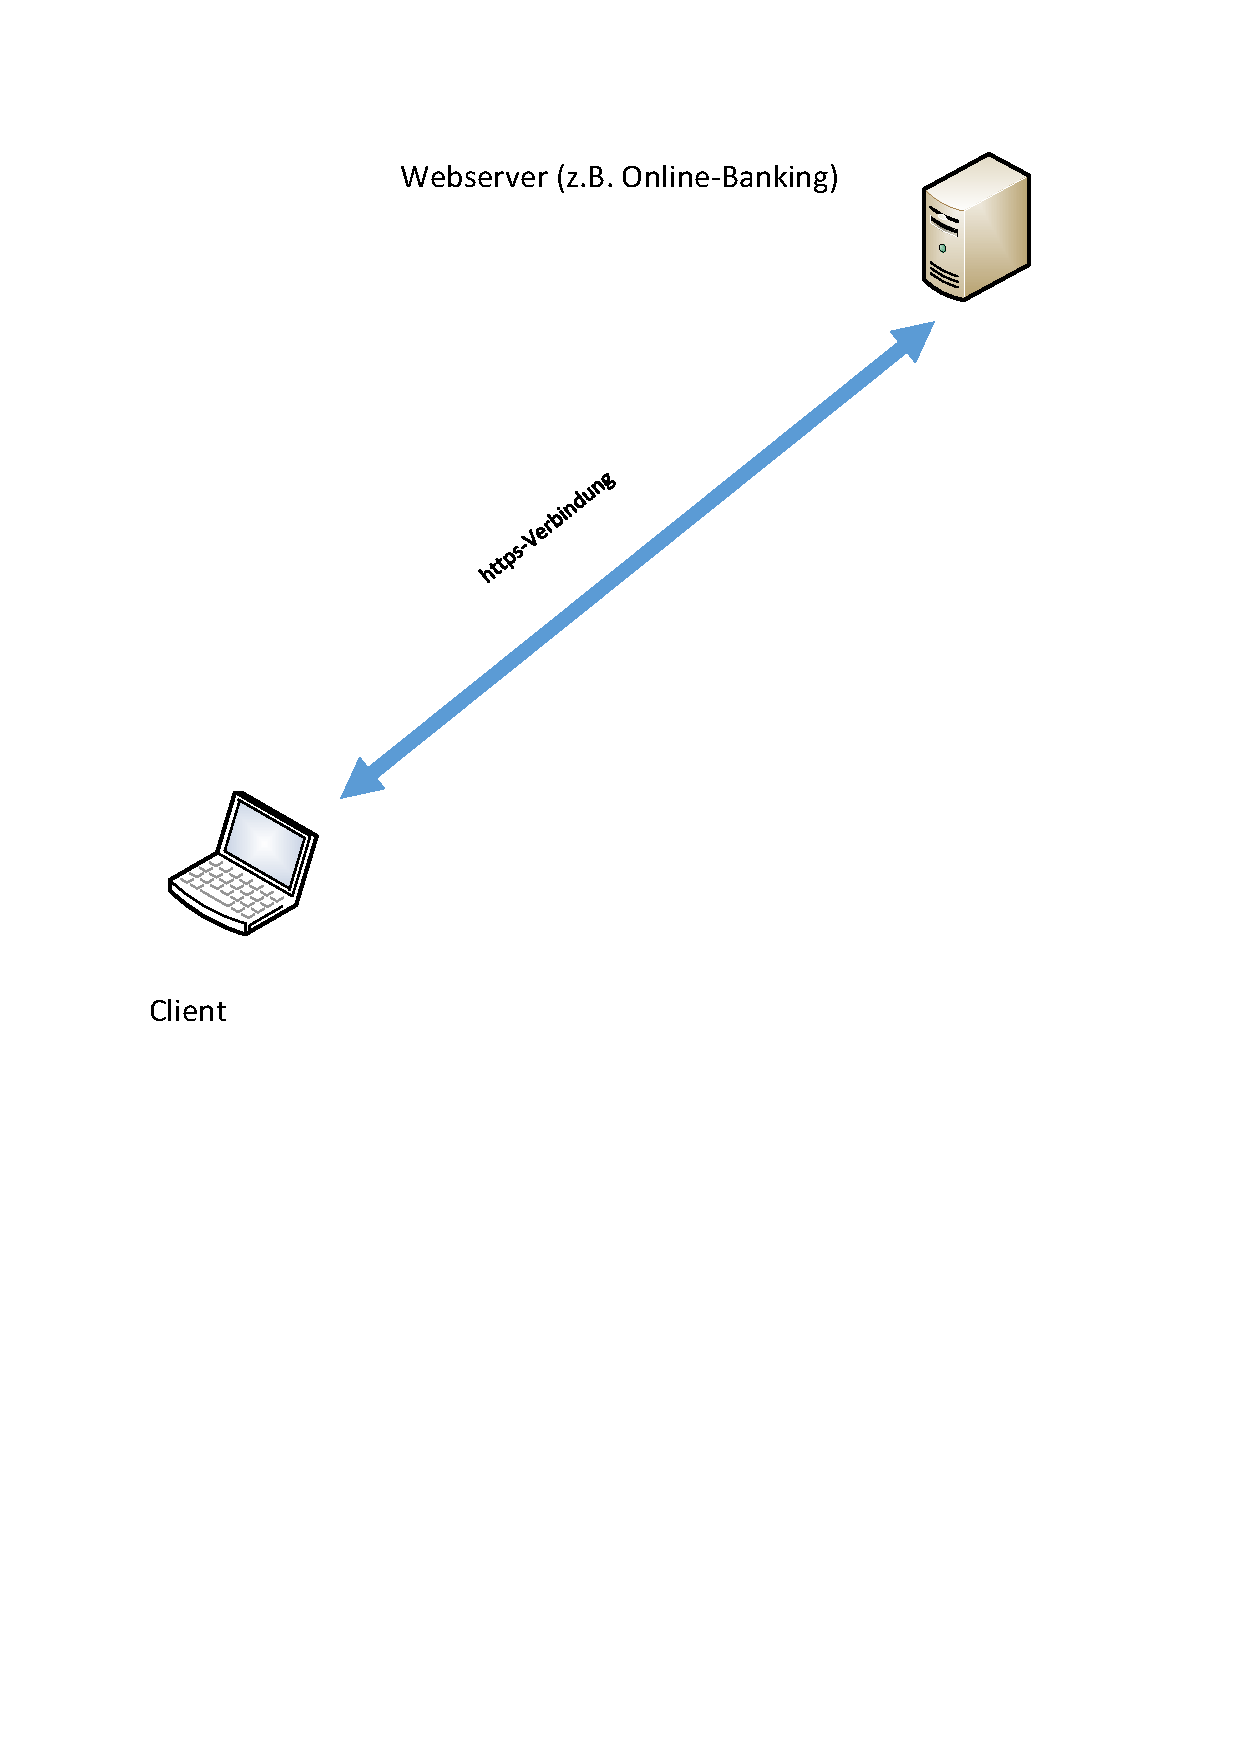
\includegraphics[width=0.6\textwidth]{bilder/https.pdf}
	\caption{Reguläre HTTPS-Verbindung zwischen Client und Server}
	\label{fig:https}
\end{figure}

\begin{figure}[h!]
	\centering
	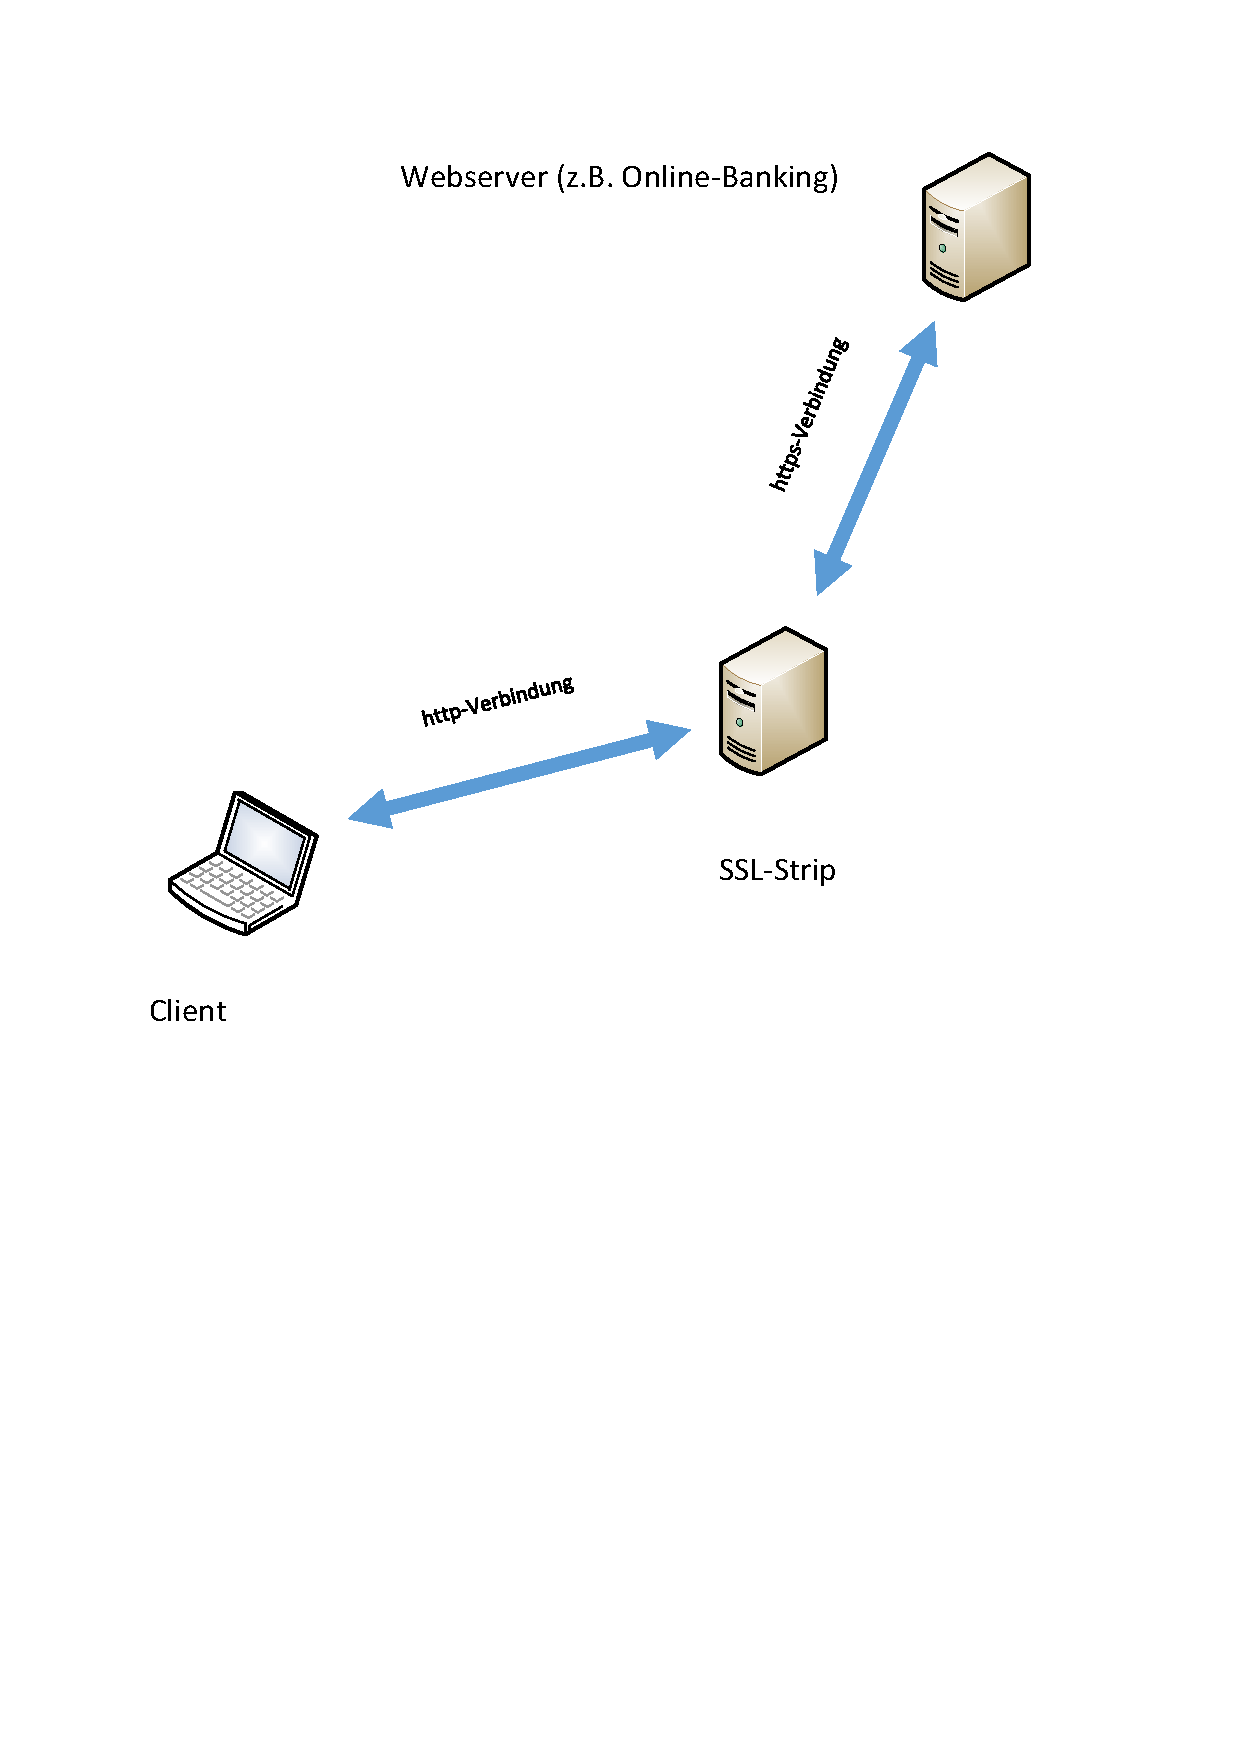
\includegraphics[width=0.65\textwidth]{bilder/sslstrip.pdf}
	\caption{SSL-Strip Szenario}
	\label{fig:sslstrip}
\end{figure}

\subsection*{Tools}
Um SSLStrip einsetzen zu können sind mehrere Schritte notwendig. Auf Kali Linux 2.0 sind alle benötigten Tools bereits vorinstalliert. \\

IP-Forwarding, also das Weiterleiten von IP-Paketen, kann durch folgende Befehle aktiviert werden:\\

\begin{lstlisting}[caption=Aktivieren von IP-Forwarding]{Name}
	sysctl -w net.ipv4.ip_forward=1
	alternativ: echo 1 > /proc/sys/net/ipv4/ip_forward
\end{lstlisting}
	

Anschließend wird ARP-Spoofing gestartet. Dies geschieht mit folgenden Befehlen:
\begin{lstlisting}[caption=Parameter für ARP-Spoofing]
arpspoof -i <interface> -t <targetIP> <gatewayIP>
Parameter:
	-i  <interface>		Angabe des Interfaces, in dem sich Angreifer und Client befinden.
	-t <targetIP>   	IP-Adresse des anzugreifenden Clients
	<gatewayIP>   		IP-Adresse des Gateways im LAN
\end{lstlisting}

Nachdem nun mittels ARP-Spoofing alle IP-Pakete vom angegriffenen Client über den Angreifer gesendet werden, müssen die umgeleiteten HTTP-Pakete via IPtables an das Tool SSLStrip weitergereicht werden. Dies geschieht mittels folgendem Eintrag:\\

\begin{lstlisting}[caption=Eintrag in IP-Tables damit HTTP-Pakete an sslstrip weitergereicht werden]
iptables -t nat -A PREROUTING -p tcp --destination-port 80 -j REDIRECT --to-port <listenPort>
Parameter:
	-t nat                 	: Firewall-Gruppe
	-A PREROUTING          	: Regel wird angewandt, BEVOR Paket geroutet wird
	-p tcp                 	: Nur TCP-Pakete
	--destination-port 80  	: Nur Pakete auf Port 80 (http)
	-j REDIRECT            	: Legt Aktion fest, also Weiterleitung
	--to-port <listenPort> 	: Port auf dem SSLStrip lauscht.
\end{lstlisting}


Nun muss noch SSLStrip selbst gestartet werden. Dies geschieht mittels folgender Eingabe:
\begin{lstlisting}[caption=Erforderliche Parameter für SSLStrip]
sslstrip -a -k -l <listenPort> -w <logpath>
Parameter:
	-s : Gesamter SSL Traffic wird gelogged
	-p : Nur SSL POST Traffic wird protokolliert
	-a : SSL- und HTTP-Traffic wird aufgezeichnet
	-k : Bestehende SSL-Verbindungen terminieren, damit diese neu aufgebaut werden
	-l : Port auf dem SSLStrip lauscht. Muss identisch zu --to-port bei iptables-Eintrag sein
	-w : Pfad in dem gehijackter HTTPS-Traffic im Klartext abgespeichert wird
\end{lstlisting}
	
\subsection*{Benutzung von SSLStrip-Skript}
Zur Automatisierung wurden vorangegangene Befehle in einem Skript automatisiert. Nachdem SSLStrip im Auswahlmenü selektiert wurde, wird zuerst nach der Netzwerkschnittstelle gefragt, in der Angreifer und Zielclient sich befinden. Anschließend wird das ausgewählte Netzwerk nach aktiven Hosts gescannt und aufgelistet. Im folgenden Schritt wird die Ziel-IP-Adresse des anzugreifenden Clients eingegeben, gefolgt von der IP-Adresse des Gateways für ARP-Spoofing. Abschließend werden die erforderlichen Konfigurationen für SSLStrip-Attacke im Hintergrund durchgeführt und der mitgeschnittene HTTPS-Verkehr im Klartext in der LOG-Datei abgerufen werden.
 
 
\subsection*{Gegenmaßnahmen}

\subsubsection*{HTTP Strict Transport Security}
HTTP Strict Transport Security ist ein Mechanismus um einem Client mitzuteilen, dass er für eine bestimmte Zeit nur verschlüsselte Verbindungen verwenden soll. Der Server übermittelt in seiner Antwort im Header, zusätzliche Informationen über die Gültigkeit der Information und ob sämtliche Subdomains ebenfalls ausschließlich verschlüsselte Verbindungen annehmen dürfen. \cite{hsts} \newpage
%Quellen:
%[1]https://de.wikipedia.org/wiki/Hypertext_Transfer_Protocol
%[2]https://de.wikipedia.org/wiki/Hypertext_Transfer_Protocol_Secure


\section{Fake IPv6 Netz}

\subsection*{Voraussetzungen}
Für diesen Angriff ist Zugang zum Netzwerk des anzugreifenden Hosts notwendig. Ebenso ist es notwendig eine gültige IPv4-Adresse aus diesem Netzwerk zu besitzen. Die Rechner des angegriffenen Netzes müssen IPv6 aktiviert haben, allerdings dürfen keine IPv6-Adressen und Routen über einen DHCP Server verteilt werden.
Der angreifende Rechner benötigt Tools um Router Advertisments im Netz zu versenden, IPv6-Adressen zu verteilen, IPv6-Adressen in IPv4-Adressen umzuwandeln sowie einen DNS Server.

\subsection*{Grundlagen}

\subsubsection*{IPv6}
IPv6 wurde eingeführt, da der IPv4 Adressraum mit 2\textsuperscript{32} (wobei nicht alle für die Adressierung verwendet werden können) Adressen zu klein geworden ist. Der Adressraum wurde auf 2\textsuperscript{128} erweitert um auch in der Zukunft genug Adressen zur Verfügung zu haben. IPv6 stellt ein vollkommen neues Protokoll dar und ist daher nicht abwärtskompatibel zu IPv4 (so wurde z.B. ARP durch das Neighbor Discovery Protocol ersetzt). 
Die Konfiguration der IPv6-Adressen erfolgt entweder via SLAAC (Stateless Address Autoconfiguration) bei der sich der Host selber eine Adresse bestehend aus dem Netzwerkpräfix und dem Interface Identifier zuweist und diese dem Netzwerk mitteilt. Eine andere Möglichkeit ist es, einen DHCP-Server für IPv6 einzusetzen. Dies hat den Vorteil, dass z.B. DNS-Adressen und Domainnamen mitkonfiguriert werden können.
Der IPv6 Netzwerkverkehr wird in einem dual-stack Netz (IPv4 und IPv6 im Parallelbetrieb) bevorzugt. Diese Eigenschaft ist die Grundlage dieses Angriffes.

\subsubsection*{Nat64}
Hierbei handelt es sich um einen Mechanismus, mit dessen Hilfe IPv6-Adressen in IPv4-Adressen (und IPv4 in IPv6) umgewandelt werden. Dies ermöglicht die Kommunikation von Rechnern aus unterschiedlichen IP-Konfigurationen. 
Die Umwandlung einer IPv4-Adresse in eine IPv6-Adresse erfolgt über eine Kapselung:
Beispiel:
\begin{itemize}
	\item IPv4-Adresse: 192.168.178.10 (Hex: C0A8:B20A)
	\item IPv6-Präfix: 2010:808:abc:FFFF::/64
\end{itemize}
Dies ergibt die Adresse: 2010:808:abc:FFFF:: C0A8:B20A. Die Umwandlung einer IPv6- in eine IPv4-Adresse stellt die umgekehrte Operation dar, es werden die letzten 8 Byte der Adresse in eine IPv4-Adresse umgewandelt.

\subsubsection*{Router Advertisment}
Mittels Router Advertisment bieten Router ihre Dienste in einem Netzwerk an. Dies geschieht entweder auf Anfrage (Router Solicitation) oder in festen Zeitabständen.

\subsection*{Szenario}
In einem IPv4 Netzwerk installiert der Angreifer seinen Rechner als IPv6 Router, DHCP-Server und Gateway. Zusätzlich stellt er einen DNS-Server bereit. Das Ziel dieses MITM-Angriffes ist, den kompletten Netzwerkverkehr (IPv4 und IPv6) über den Rechner des Angreifers laufen zu lassen. Hierfür wird Nat64 eingesetzt, das angegriffene Netz kommuniziert dadurch nur noch über IPv6, die Umwandlung in IPv4-Adressen erfolgt am Rechner des Angreifers. Abbildung \ref{fig:fakeIpv6_szenario} stellt schematisch das angegriffene Netz inklusive Rechner des Angreifers dar.
\begin{figure}[h!]
	\centering
	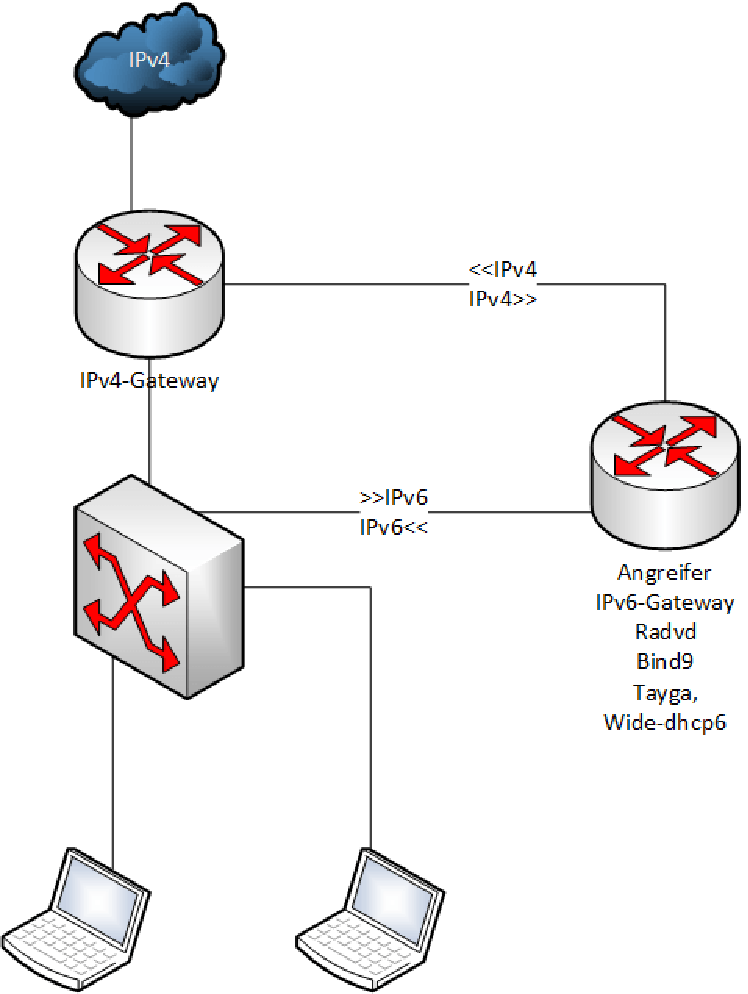
\includegraphics[width=0.8\textwidth]{bilder/fakeIPv6/fakeIpv6_szenario.pdf}
	\caption{Schematische Darstellung des angegriffenen Netzes}
	\label{fig:fakeIpv6_szenario}
\end{figure}

\subsection*{Technisches}
Sobald der Angriff gestartet wird, erhalten die Clients im angegriffenen Netz eine IPv6-Adresse, die IPv6-Adressen des DNS-Servers und des Gateways des Angreifers. Diese werden durch vom Tool radvd versendete Router Advertisments konfiguriert. Da der IPv6-Verkehr vom Betriebssystem priorisiert behandelt wird, richten sich sämtliche DNS Anfragen an den DNS-Server des Angreifers (der „alte“ DNS-Server hat nur eine IPv4-Adresse). 
Dieser liefert immer eine AAAA-Antwort. Dabei ist es egal ob eine IPv4- oder IPv6-Adresse angefragt wurde, da der Angreifer Adressen mittels Nat64 übersetzen kann. Da alle Hosts des angegriffenen Netzes IPv6-Adressen bei DNS Anfragen gemeldet bekommen, läuft der Netzwerkverkehr immer über das IPv6-Gateway, also über den Rechner des Angreifers. Dieser kann z.B. mit Wireshark den Netzwerkverkehr mitlesen.

\subsection*{Erklärung der verwendeten Skripte und Tools}

\subsubsection*{Radvd}
Der Router Advertisment Deamon (radvd) ist ein Programm, welches auf IPv6 Routern läuft. Es sendet zum einen periodisch Router Advertisments (RAs) aus. Zum anderen reagiert es auch, wenn per Router Solicitation angefragt wird. Die Installation erfolgt aus den Debian-Paketquellen. Zusätzlich muss für das Senden von RAs das IPv6 Forwarding aktiviert sein:
\lstset{language=bash}
\begin{lstlisting}[
	basicstyle=\footnotesize,
]
apt-get install radvd
echo 1 \textgreater /proc/sys/net/ipv6/conf/all/forwarding
\end{lstlisting}

Die Konfigurationsdatei liegt unter \textit{/etc/radvd.conf} (muss vor der ersten Ausführung des Python Skripts noch nicht vorhanden sein). In Tabelle \ref{tab:radvdConfig} wird der Inhalt dieser Datei erläutert.
\begin{lstlisting}[
	basicstyle=\footnotesize,
]
interface eth0 {
	AdvSendAdvert on;
	MinRtrAdvInterval 3;
	MaxRtrAdvInterval 10;
	AdvHomeAgentFlag off;
	AdvOtherConfigFlag on;
	prefix 2001:06f8:0608:fab::/64 {
		AdvOnLink on;
		AdvAutonomous on;
		AdvRouterAddr on;
	};
};
\end{lstlisting}

\begin{table}
	\centering
		\begin{tabular}{lp{9cm}}
			Konfigurationselement & Bedeutung \\ \hline
			interface eth0 & Legt das Interface fest für das RAs versendet werden sollen. \\
			AdvSendAdvert on & Aktiviert das Senden von RAs und die Antwort auf Router Solicitations. \\
			MinRtrAdvInterval 3 & Minimalzeit zwischen ausgesendeten RAs in Sekunden. Betrifft nur das periodische Senden, nicht die Antwort auf Router Solicitations. \\
			MaxRtrAdvInterval 10 & Maximalzeit zwischen ausgesendeten RAs in Sekunden. Betrifft nur das periodische Senden, nicht die Antwort auf Router Solicitations. \\
			AdvHomeAgentFlag off & Der Router kann nicht als Home-Agent für Mobile-IPv6 verwendet werden. \\
			AdvOtherConfigFlag on & Stellt sicher, dass nicht-adressbezogene Konfigurationsinformationen mitgeteilt werden sollen. \\
			prefix 2001:06f8:0608:fab::/64 & Legt das Netzwerkpräfix fest, das die Hosts nutzen sollen. \\
			AdvOnLink on & Legt fest, dass die Bereitstellung on-link erfolgt (ohne Hop über weiteren Router). \\
			AdvAutonomous on & Das Präfix kann für selbstständige Adress Konfiguration verwendet werden. \\
			AdvRouterAddr on & Legt fest, dass die Adresse des Interfaces und nicht das Präfix gesendet wird.  \\
		\end{tabular}
	\caption{Erläuterung der radvd Konfiguration}
	\label{tab:radvdConfig}
\end{table}
\FloatBarrier
\subsubsection*{Bind}
Als DNS Server kommt Bind (Berkeley Internet Name Domain) zum Einsatz. Dieser offene DNS-Server ist für alle gängigen Betriebssysteme verfügbar und genießt eine hohe Verbreitung. Die Installation erfolgt aus den Debian-Paketquellen:
\lstset{language=bash}
\begin{lstlisting}[
	basicstyle=\footnotesize,
]
apt-get install bind9
\end{lstlisting}

Die Konfigurationsdatei liegt unter \textit{/etc/bind/named.conf.options} (muss vor der ersten Ausführung des Python Skripts noch nicht vorhanden sein). In Tabelle \ref{tab:bindConfig} wird der Inhalt dieser Datei erläutert.
\begin{lstlisting}[
	basicstyle=\footnotesize,
]
options {
	directory "/var/cache/bind";
	forwarders {
		8.8.8.8
	};
	dnssec-validation auto;
	auth-nxdomain no;
	listen-on-v6 { any; };
	allow-query { any; };
	dns64 2001:db8:1:FFFF::/96 {
		clients { any; };
		exclude { any; };
	};
};
\end{lstlisting}

\begin{table}
	\begin{tabular}{lp{9cm}}
		Konfigurationselement & Bedeutung \\ \hline
		directory "/var/cache/bind" & Verzeichnis in dem sich die Zonendaten befinden. \\
		forwarders & Alle aufgeführten IP-Adressen stellen DNS-Server dar. Bind muss die Anfrage an einen dieser Server weiterreichen. \\
		dnssec-validation auto & Bind versucht Antworten aus DNSSEC gesicherten Zonen zu validieren. „auto“ gibt dabei an, dass Binds default Sicherheitseintrag verwendet wird. \\
		auth-nxdomain no & Der DNS-Server darf keine autoritativen Antworten senden (z.B., wenn er im Cache die Information gespeichert hat, dass eine Adresse nicht über den Nameserver ihrer Zone existiert) \\
		listen-on-v6 \{ any; \} & Bind lauscht auf Port 53 (default) auf Anfragen aus allen Netzen. \\
		allow-query \{ any; \} & Clients dürfen aus allen Netzen heraus Anfragen an den DNS-Server stellen. \\
		dns64 2001:db8:1:FFFF::/96 & Die folgenden Punkte legen das Verhalten von dns64 für das Netz 2001:db8:1:FFFF::/96 fest. \\
		clients \{ any; \} & Dns64 ist für alle Clients des Netzes aktiv. \\
		exclude \{ any; \} & Dns64 verwirft sämtliche AAAA-Antworten, fragt A-Einträge an und bildet daraus neue AAAA-Antworten (siehe Nat64). \\
	\end{tabular}
	\caption{Erläuterung der Bind Konfiguration}
	\label{tab:bindConfig}
\end{table}

\FloatBarrier

\subsubsection*{Tayga}
Bei Tayga handelt es sich um eine Nat64 Implementierung für Linux-Systeme. Es legt eine neue, virtuelle Netzwerkschnittstelle an um IPv4- in IPv6-Adressen umzuwandeln. Die Installation erfolgt aus den Debian-Paketquellen:
\lstset{language=bash}
\begin{lstlisting}[
	basicstyle=\footnotesize,
]
apt-get install tayga
\end{lstlisting}


Die Konfigurationsdatei liegt unter \textit{/etc/tayga.conf} (muss vor der ersten Ausführung des Python Skripts noch nicht vorhanden sein). In Tabelle \ref{tab:taygaConfig} wird der Inhalt dieser Datei erläutert.
\begin{lstlisting}[
	basicstyle=\footnotesize,
]
un-device sBnat64
ipv4-addr 192.168.255.1
prefix 2001:db8:1:FFFF::/96
dynamic-pool 192.168.255.0/24
\end{lstlisting}

\begin{table}
	\centering
		\begin{tabular}{lp{9cm}}
			Konfigurationselement & Bedeutung \\ \hline
			tun-device sBnat64 & Legt den Namen des virtuellen Interfaces fest. \\
			ipv4-addr 192.168.255.1 & IPv4-Adresse, die von Tayga verwendet wird. Diese darf nicht Teil des angegriffenen Netzes sein. \\
			Prefix 2001:db8:1:FFFF::/96 & Verwendetes Präfix um IPv4-Adressen in IPv6-Adressen zu kapseln. \\
			dynamic-pool 192.168.255.0/24 & Legt einen Adresspool fest, welcher für Mapping von IPv6-Adressen verwendet wird, die nicht dem Präfix entsprechen. \\
		\end{tabular}
	\caption{Erläuterung der tayga Konfiguration}
	\label{tab:taygaConfig}
\end{table}

\FloatBarrier

Durch Ausführen von 
\lstset{language=bash}
\begin{lstlisting}[
	basicstyle=\footnotesize,
]
/usr/sbin/tayga --mktun
\end{lstlisting}

wird das virtuelle Interface angelegt. Mit \textit{ifconfig} kann die Konfiguration eingesehen werden (Abb. \ref{fig:tunInterface}). 
\begin{figure}[h!]
	\centering
	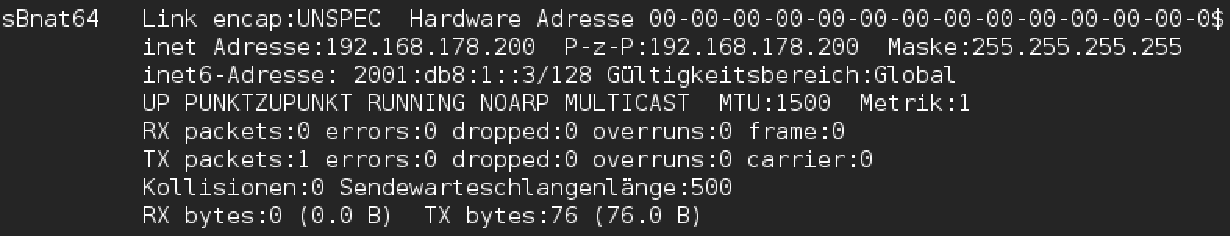
\includegraphics[width=0.80\textwidth]{bilder/fakeIPv6/tunInterface.pdf}
	\caption{Ifconfig-Ausgabe des virtuellen Interfaces}
	\label{fig:tunInterface}
\end{figure}


\subsubsection*{Wide-dhcpv6}
Als IPv6-DHCP-Server kommt wide-dhcpv6 zum Einsatz. Hierbei handelt es sich um eine open-source Implementierung von DHCP für IPv6. Die Installation erfolgt aus den Debian-Paketquellen:
\lstset{language=bash}
\begin{lstlisting}[
	basicstyle=\footnotesize,
]
apt-get install wide-dhcpv6-server
\end{lstlisting}

Die Konfigurationsdatei liegt unter \textit{/etc/wide-dhcpv6/dhcp6s.conf} (muss vor der ersten Ausführung des Python Skripts noch nicht vorhanden sein). In Tabelle \ref{tab:wideDhcpConfig} wird der Inhalt dieser Datei erläutert.
\begin{lstlisting}[
	basicstyle=\footnotesize,
]
option domain-name-servers 2001:db8:1::2;
option domain-name "securityWorkbench";
interface eth0 {
	address-pool addrPool 3600;
};
pool addrPool {
	range 2001:db8:1:CAFE::10 to 2001:db8:1:CAFE::0240;
};

\end{lstlisting}

\begin{table}
	\centering
		\begin{tabular}{lp{9cm}}
			Konfigurationselement & Bedeutung \\ \hline
			option domain-name-servers 2001:db8:1::2 & Legt die IPv6-Adresse des DNS-Servers fest. \\
			option domain-name "securityWorkbench" & Name der Domain. \\
			interface eth0 & Setzt das DHCP-Interface auf eth0. \\
			address-pool addrPool 3600 & Legt den Adresspool für DHCP auf „addrPool“fest. 3600 stellt die Gültigkeit in Sekunden dar.  \\
			pool addrPool & Legt einen neuen Adresspool (addrPool) an. \\
			range 2001:db8:1:CAFE::10 to 2001:db8:1:CAFE::0240 & Gibt den Adressbereich des Adresspools an. \\
		\end{tabular}
	\caption{Erläuterung der wide-dhcp6 Konfiguration}
	\label{tab:wideDhcpConfig}
\end{table}

\FloatBarrier


\subsubsection*{Iptables}
Zusätzlich müssen noch einige Iptables Einträge vorgenommen werden (Tab. \ref{tab:IptablesEintraege}).
\begin{table}
	\centering
		\begin{tabular}{p{6cm}p{9cm}}
			Eintrag & Auswirkung \\ \hline
			/sbin/iptables -I FORWARD -j ACCEPT -i sBnat64 -o eth0 & Alle Pakete, die an Interface sBnat64 eingehen und über Interface eth0 versendet werden, werden akzeptiert. \\ \hline
			/sbin/iptables -I FORWARD -j ACCEPT -i eth0 -o sBnat64 -m state --state RELATED,ESTABLISHED & Alle Pakete, die an Interface eth0 eingehen, über Interface sBnat64 versendet und die zu einer bestehenden Verbindung oder mit einer bestehenden Verbindung verwandt sind (z.B. ein ICMP Fehler) werden akzeptiert. \\ \hline
			/sbin/iptables -t nat -I POSTROUTING -o eth0 -j MASQUERADE & Pakete, die über das Interface eth0 versendet werden und auf die NAT angewendet wird, werden nach dem Routen (aber vor dem Versenden) maskiert. Der Router setzt seine eigene Adresse als Quelladresse ein. \\ \hline
			/sbin/ip6tables -A OUTPUT -p icmpv6 --icmpv6-type 1 -j DROP & ICMPv6 Pakete werden verworfen. \\
		\end{tabular}
	\caption{Iptables Einträge}
	\label{tab:IptablesEintraege}
\end{table}

\subsection*{Benutzung des Python Skripts}
\begin{enumerate}
	\item Im Hauptmenü des Skriptes den Punkt „Fake IPv6 Network“ wählen. Anschließend „Start Attack“ auswählen.
	\item Das Interface angeben, welches für den Angriff verwendet werden soll. Bei einfacher Bestätigung mit Enter, ohne ein Interface angegeben zu haben, wird standardmäßig das Interface eth0 verwendet.
	\item Anschließend werden alle verwendeten IPv4-Adressen des angegriffenen Netzwerkes aufgelistet. Es ist eine nicht-verwendete Adresse für das virtuelle tayga-Interface auszuwählen.
	\item Der Angriff läuft, die Auswirkungen lassen sich in Wireshark beobachten.
	\item Drücken von „Enter“ beendet den Angriff.
	\item Soll der Angriff erneut gestartet werden, empfiehlt es sich den angreifenden Rechner neu zu starten um alle nicht persistenten Einstellungen zu verwerfen.
\end{enumerate}
Ausgabe des Programms während des Angriffs:
\begin{figure}[h!]
	\centering
	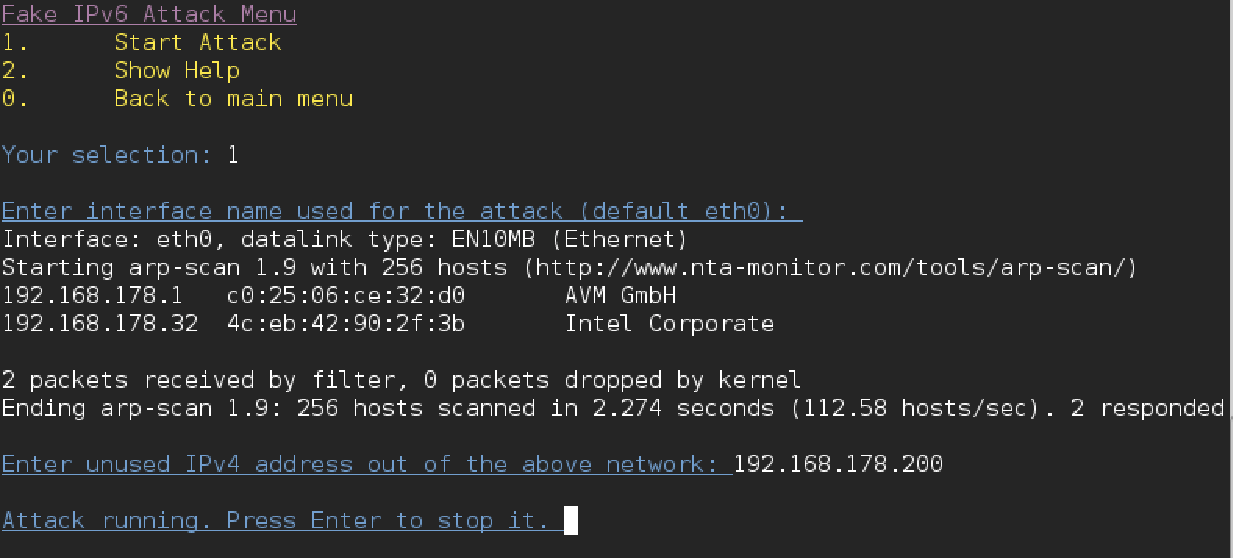
\includegraphics[width=0.80\textwidth]{bilder/fakeIPv6/fakeIPv6menu.pdf}
	\caption{Konsolenausgabe des Angriffs}
	\label{fig:fakeIPv6menu}
\end{figure}


\subsection*{Gegenmaßnahmen}
Eine Möglichkeit das Netzwerk gegen diesen Angriff zu schützen ist, die automatische IPv6-Konfiguration zu verbieten und stattdessen auf manuelle Konfiguration umzuschalten. \\
RA-Snooping bietet eine weitere Möglichkeit. Hierbei werden auf Layer-2 Switches RAs analysiert. RAs aus falschen Quellen werden blockiert oder verworfen. \\
Den sichersten Schutz gegen diesen Angriff bietet das Deaktivieren von IPv6. Da nur IPv4 verwendet wird, stellt aktiviertes, aber nicht konfiguriertes IPv6 nur eine weitere Sicherheitslücke dar.
